%!TEX root =  ../main.tex

\mychapters{Functions}{functions}{\chapdir/pics/Mountain-type_Woodland_Caribou}


Functions are the central objects of investigation in many subdivision of mathematics today, and
are very effective means of representing real-life phenomena. For example, in any given year, 
there is one population of
deer in a certain forest.  Would it make sense for a forest ranger to answer you two numbers when
you ask how many \textit{Rangifer tarandus} (caribou) exist in a given range, at a certain time?


\begin{figure}[h]
\centering
\begin{tikzpicture}
    \begin{axis}%
    [
        %grid=major,     
        xmin=0,
        xmax=12,
        axis x line=bottom,
        ytick={0,10,...,100},
        ymax=110
       % axis y line=middle,
    ]
        \addplot%
        [
            blue,%
            mark=none,
            samples=100,
            domain=0:12,
        ]
        (x,{1+100/(1+exp(-x+5))});
    \end{axis}
\end{tikzpicture}
\caption{Population of caribou over time}
\end{figure}

How do we model phenomena in the world?  Is it reasonable to expect
caribou population to follow a curve such as the above figure?  How can we 
extract information from a graph like this?  If actual measurements diverge some
from the expectation established by the curve, are they \emph{wrong}?  Are functions
better tools than relations?  What else could there be?

\newpage
\chapterminitoc

This chapter is entitled functions.  You have been studying functions for several years now,
and should be familiar with function notation.  It is also possible to present functions 
graphically, or in a table.  Lastly, we may write or speak a verbal description of a function,
but this requires technical jargon, with which you are just starting to become familiar.

Hopefully, your time in algebra classes until now has helped you achieve a basic familiarity
with certain elementary or parent functions.  You will need to recognize them in each
of the four ways.  These prototypical versions can be moved or stretched as needed.  They
can also be mirrored or reflected.  This should naturally lead to the observation that some
graphs are unchanged under certain types of reflection.

Lastly, we will introduce the rich and vast field of taking numerical data and generating
an algebraic equation, called regression.  


%								1 - 1
\newpage
\invisiblesection{Representations}
\marginlessinput{\chapdir/0101p}
\newpage
%!TEX root =  ../main.tex

\subsection{Numerical, Graphical, Algebraic, and Verbal}


\objective{Use functions defined numerically, graphically, algebraically, or verbally.}



A \gls{function} is a relation that uniquely associates members of one \gls{set} 
with members of another set.  
More simply, a function connects members of a \gls{domain} to members of a \gls{range}, 
with the proviso that each element in the domain maps onto only one element in the range.  
When graphing a function, it is customary to plot the \emph{input} or \gls{independent variable} 
on the $x$-axis (going left to right), and the \emph{output} or \gls{dependent variable} on 
the $y$-axis (going down to up).  The independent variable is so-called because it may 
be arbitrarily chosen from within the domain.  The dependent 
variable is then forced to be a particular value (by the function).

\subsubsection{Numerically}
Typically, information is gathered about the physical world as \gls{discrete} numbers, 
occurring at fixed points. Such information may be represented as in  table ~\ref{tab:Numerically}.

\columntable[-0.75in]{1.6in}{
  \begin{tabular}{ lr }
  \hline
  \textbf{x} (months since) & \textbf{y} (100's of \$)\\
  \hline
  0 & 1200.00 \\
  1 & 840.00 \\
  10 & 1680.24 \\
  16 & 2072.98 \\
  23 & 2264.72 \\
  36 & 4303.93 \\
  48 & 6770.53 \\
  \hline
  \end{tabular}
   }{Monthly income represented numerically\label{tab:Numerically}}
    
    
\subsubsection{Graphical}
A helpful way to visualize relationships between input and output 
sets is a \gls{graph} of the function.  Similar techniques
include diagrams (see Figure for an example) and maps (see Figure for an example).  
``Mapping diagrams'' blur the line between numerical and graphical data 
(see Figure ~\ref{fig:graphically} for an example).

\begin{figure}[h]
\centering
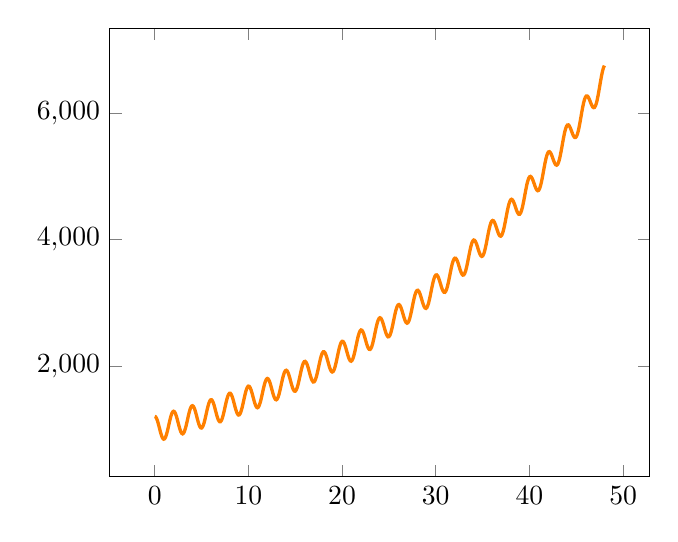
\begin{tikzpicture}
\begin{axis}[samples=500,domain=0:48,restrict y to domain =0:8500]
\addplot[very thick,orange ]plot (\x, {1000*(pow(1.04,\x))+200*cos((\x r)*3.1415)});
\end{axis}
\end{tikzpicture}
\caption[Graph]{Monthly Income  - Graphically\label{fig:graphically}}
\end{figure}


\subsubsection{Algebraically}
Typically, graphs come from humans or machines plotting many, 
many points derived from an \gls{algebraic} formula.
Algebra is a powerful tool for describing natural phenomena, 
but it cannot do everything.  Important numbers
--- such as \gls{pi} or $e$ --- cannot be defined via algebraic techniques.  
Worse, many confuse manipulation of the symbols with actually mathematics.
However, the symbols are very concise, as you might see in Tab.~\ref{tab:algebra}.

\columntable[-0.75in]{0.3in}{
\begin{center}
$y=1000\cdot1.04^x+200\cos(\pi x)$.
\end{center}}
{Monthly Income - Algebraically\label{tab:algebra}}



\subsubsection{Verbally}
Ordinary language serves us well most of the time, with an average level of 
precision and an average level of
emotional content.  Sometimes, however, what we wish to convey is more 
meaningful and deep than
regular wording can describe.  Conversely, we might wish to exclude a whole 
host of meanings, and narrowly
zoom in on precise terminology, in order to avoid error to the fullest extent possible
(see Fig.~\ref{fig:lol}).

\marginfig[-0in]{\chapdir/pics/levelsoflanguage}{Levels of language\label{fig:lol}}

Most of us encounter poetic language\index{language} in the form of songs, since ours is an 
age sadly bereft of
poetry, something that was not true a century ago or more.  Another common 
phenomenon is to meet 
technical language when it is not expected or welcome, such as when we read the 
instruction manual for new
hardware or legal documents.  However, such documents are typically not aiming at 
easy comprehension, but
precision.  Like most jargon, they tend to use mostly ordinary words in extraordinary 
ways, similar but opposite
to poetry.

Mathematics is no difference.  This textbook is a formal setting, and as such, 
it uses technical language, carefully
choosing each word according the conventions and definitions ``in house''.  
As you cross the threshold into the
beginning stages of advanced mathematics, you must cultivate the skill of 
using this ``jargon'', something you 
do not ordinarily do.  It may help your comprehension to paraphrase 
what you are learning into the ``vernacular'',
but you should not consider a topic concluded until you are able to 
re-articulate the mater in mathematical terminology.
For example, the equation above might be described as in Fig.~\ref{fig:verbally}.

\begin{figure}
\emph{The income ($y$) may be modeled by the number of months since 
inception ($x$) as a sinusoid with an amplitude of 200, a period of 2, and a
midline of an exponential growth rate of 4\% beginning at \$1,000.}
\caption{Monthly Income - Verbally\label{fig:verbally}}
\end{figure}

\subsubsection{Mathematical Models}
Functions that can be used to make predictions and 
interpretations of real-world phenomena are called \textbf{mathematical
models}.
It is important to be clear which variable is being used as input 
and which is output, so that a meaningful
relationship between independent and dependent variables 
can be ascertained.  In the model of income above,
time does not depend upon money, but rather money upon time.  
The domain of the function is the initial time
index of zero until four years later, so in months $0\le x \le 48$.  
The income varies from as low as \$840 but
generally goes up from there, so the range is $y\ge840$.

\begin{example}
	\exProblem
There are only so many hours in a day.  If you decide to stay up \emph{all} night studying, 
you will surely get
a bad grade on the test tomorrow, due to sleep deprivation.  
Sketch a reasonable graph showing hours spent studying the day before
a test and the grade you will get on said test.  Give the domain and range of the function.

	\exSolution
One cannot possibly get less than zero hours of sleep, and presumedly around 
12 or so hours of sleep is
long enough to have slept through the exam and angered one's parents!  
Test scores are typically measured in percents, ranging from 0 to 100.

\marginfig[-1.8in]{\chapdir/pics/sleep.png}{Possible graph of sleep vs. grade}
\end{example}

~\vfill
\newpage
\subsection{Exercises}
\marginlesspdf{\chapdir/0101xA.pdf}
\marginlesspdf{\chapdir/0101xB.pdf}
\marginlesspdf{\chapdir/0101xC.pdf}



%								1 -2
\newpage
\invisiblesection{Types}
\subsection{Pick x, Find y}
\marginlesspdf{ch01/0102p.pdf}
\newpage
%!TEX root =  ../main.tex


\objective{Connect names of types of equations with graphs.}


We have said that a function is a relation of inputs to outputs, with no more than one output per input.  
We have learned that functions can be defined graphically, algebraically, numerical, or verbally.
A function that is defined by an algebra equation usually has a descriptive name.
In this section, we will look at several groupings of various functions, some of which you should
be very familiar with, and some of which may be new.


You might be used to seeing a  \gls{graph} of certain equations, written algebraically with $y$ in terms
of $x$, like $y=x$.  These have then been graphed on the Cartesian plane, as a continuous curve,
with each point corresponding to an ordered pair, $(x,y)$.  Leonhard Euler created much of the notation
we use today, including \emph{function notation}: $y=f(x)$.

\marginfig[-0in]{\chapdir/pics/Linear_Function_Graph.png}{Linear functions.\label{fig:LinearFunction}}
\subsubsection{Linear}
One of the most obvious things to see is a straight line.  
Humans create straight lines seemingly more often
than anything else.  Hence, lines can feel unnatural or reassuring.  
What are some of the properties of lines?
How might two lines be the same?  How might they differ?  

\marginfig[-0in]{\chapdir/pics/AndraGrad-4}{A quadratic function is a polynomial of degree two.}
Lines could have the same slope, and therefore never run into each other.  
They would only be distinguished by their
heights.  For convenience, we measure the height of a \gls{linear} function 
in Analytic Geometry by its starting value, its $y$ when $x$ 
equals zero.  Conversely, these starting locations might be the same and 
slope might be different.  You have learned \index{linear!intercept form}
to distinguish these two different variables as $m$ and $b$, as in $y=mx+b$, and we shall see
that it is expedient to distinguish them \textbf{constant} functions, $y=k$.
\index{constant!function}

\subsubsection{Quadratic}
Many things in our world operate over two dimensions, such as gravity.  
Hence, Newton find that the force
of two objects upon each other is proportional to the \emph{square} of their distance.  
Squares graphed make a
\textbf{parabola}, a word reference the path of a falling or thrown object.  
Algebraically, we can see all such shapes\index{quadratic!standard form}
have an equation of the form $y=ax^2+bx+c$, which is called \gls{quadratic}.  
You should already know a great deal about quadratics from previous classes.

\paragraph{Power}
As more dimension interact, the exponent on $x$ can become very 
complicated, and even fractional.  We can generalize\index{power function!standard form}
from $y=x$ to $y=x^2$ and $y=x^3$ to $y=a\cdot x^b$.  We shall study them in more depth
in chapter 5.

\paragraph{Polynomial}
A sum of power functions with whole number exponents is called a
\textbf{polynomial}.  Such equations are among the most well-studied
areas in mathematics.  A polynomials divided by a polynomial is called
a \textbf{rational function}.  Both are the subject of chapter 6.
\index{polynomial}\index{rational function}

\subsubsection{Exponential}
\marginfig[-0in]{\chapdir/pics/2^x_function_graph}{$2^x$ is an  exponential function}
Quantities that experience the same percentage growth or decay 
year over year look similar in the algebra: $x$ is in
the exponent, and hence such an equation is called an \gls{exponential} function.  The general form
is $y=a\cdot b^x$.  \index{exponential function!standard form}
The ``opposite''\footnote{There are \emph{many} things 
which could be called `opposite'
in mathematics, so this is not technical language.  We will define `inverses' of functions in 4.4.} of such a 
function is a called a \gls{logarithm}, and we will follow the TI-8* for now and use the generic equation
$y=a+b\ln{x}$.  \index{logarithmic function}

\subsubsection{Periodic}
Many phenomena is nature reoccur the same way at regular intervals.  Such functions are said to be 
\textbf{periodic}.
We will  study `simple harmonic motion', which comes from components of motion in circles, in section III,
Trigonometric Functions.  For now\footnote{Later, we
will factor the ``inside'', but this first kind is the sort produced by your grapher.}, use the general equation $y=a\cdot\sin(bx+c)+d$.\index{sine function}

\inlinefig{\chapdir/pics/Periodic_function_illustration.png}{\label{fig:periodic}A periodic function is so called because it repeats at a given interval, called the period (P).}

\newpage
\subsection{Exercises}
in Kuta
~\vfill


%								1 - 3
\newpage
\invisiblesection{Translations and Dilations}
\subsection{Multiplying and Adding Functions}
\marginlesspdf{ch01/0103pA.pdf}
%\newpage
\marginlesspdf{ch01/0103pB.pdf}
\newpage
%!TEX root =  ../main.tex
\subsection{Inside vs. Outside}


\objective{Produce and decipher translations and dilations of functions.}


\subsubsection{``Outside'' Operations}
How would you triple the output of a function?  How would you add four the output of a function?
Because function notation means ``perform the operation of the function upon the input'', we must
write the operators we described \emph{to the right} of the function operation, written $f(x) \cdot 3$
and $f(x) + 4$ respectively.  Normally, multiplicative operators are written on the left, without
an intervening symbol.  Because addition is commutative, it may be written on the left as well.

\paragraph{Addition}
\marginfig[-1in]{\chapdir/pics/verticaltranslation}{Vertical translation is outside addition.}
What is the graphical effect of the algebraic operation, $f(x) + 4$?  Let us build up a visual picture
numerically at first.

\emph{adding moves it up, negatives move it down.  Multiplication by $>1$ makes it taller.
$(0,1)$ makes it shorter.  All relative to the x-axis.}

\begin{example}{Outside Transformations}
	\exProblem
$r(x)=\sqrt[3]{x}$ and $s(x)=\frac{1}{2}r(x)+3$.  In what ways does the graph of
$s(x)$ differ from $r(x)$?

	\exSolution
up 3, half as tall
\end{example}
\index{transformation!translation}

\paragraph{Multiplication}
Multiplication also behave as one might expect, effecting $y$ in a directly-proportional way.
For example, regardless of what $f(x)$ is (excepting 0), then the graph of $3\cdot{}f(x)$
with be three times taller, a vertical dilation of 3.

\subsubsection{``Inside'' Operations}
Things done ``inside'' are done \emph{before} the function operates on the domain.  This means
graphically they will effect $x$.  However, their effect is quite curious, typically being the 
\emph{opposite} of what one might expect.

For example, consider the quadratic function $f(x)=x^2$, and a transformation of it, $g(x)=f(x+4)$.
We can see that the +4 is on the ``inside'', and we know that 4 is added to members of the domain
before they are plugged in to the function.  This means -4 will become 0 before it is squared.
Another way to say this that what used to be outputted at $x=0$ will now be outputted at $x=-4$.

This opposite effect also applies to dilations.  When we multiply the inside of a function by 2, it does
not produce a graph twice as wide, but \emph{half}.

\begin{example}{Inside Transformation}
	\exProblem
Consider the continuous function $f(x)$ given by the graph (looks like a radical sign).
Describe and graph the continuous $g(x)$, when $g(x)=f(2x-2)$.  What would be a more
informative way to write $g(x)$ in terms of $f(x)$?

	\exSolution
It's half as wide and left 1.  $f(2(x-1))$ would be more transparent.
\end{example}
\index{transformation!dilation}

In summary, $f(x) + d$ will shift the graph $d$ units to the right.  $f(x+c)$ will shift the graph
$c$ units to the left.  $a\cdot{}f(x)$ will make the graph $a$ times taller.  $f(b\cdot{}x)$ will
make the graph $b$ times skinnier.

~\vfill

\newpage
\subsection{Exercises}
in Kuta
~\vfill


%								1 - 4
\newpage
\invisiblesection{Reflections and Symmetries}%
\marginlessinput{ch01/0104p}
\newpage
%!TEX root =  ../main.tex
\subsection{Reflection}


\objective{Produce reflections of functions and describe their symmetry.}


As you know, multiplying numbers by $-1$ produces the additive opposite: negative values
become positive and positives become negative.  Zero is unaffected, being neither positive
nor negative.  The same principle applies to functions.  What would it look like to ``flip'' all
$x$ values?  $y$ values?

\paragraph{``Outside''}
$-f(x)$ is a reflection over the $x$-axis, leaving $x$'s untouched, and making $y$'s opposite.

We can obtain both the original and reflection across the $x$-axis by writing $\pm f(x)$.  Why
is that not a function?

\paragraph{``Inside''}
$f(-x)$ is a reflection over the $y$-axis, leaving $y$'s untouched, and making $x$'s opposite.

Does the ``opposite'' rule of inside transformations apply or not to the negative on the inside?
\index{transformation!reflection}


\subsection{Symmetry}
\paragraph{Even}\index{even functions}
\marginfig[-0in]{\chapdir/pics/Playing_card_spade_A.png}{The ace of spades (or of clubs or hearts) displays even symmetry about its center.}
Sometimes, multiplying by a negative makes no difference.  In mathematics, this can be very 
helpful to know.  Functions that are the same left-to-right and right-to-left are called \textbf{even}.
Can you guess why?  Aren't only numbers even (or odd)?



\begin{derivation}{Even Functions}
An even function has the property $f(x)=f(-x)$ for every $x$ in its domain.
\end{derivation}



Among the more basic functions are power functions.  We will study them in great depth in
chapter 5.  The names ``even'' and ``odd'' come from the similar behavior of $x^n$ when
$n$ is even or odd.

Notice that evenness has the visual appearance of putting a mirror on the $y-$axis.  Did you 
know human beings are made to find such left-right symmetry appealing?  Study the faces of
attractive people, and you will find evenness to be a rule of thumb. 



\begin{derivation}{Odd Functions}\index{odd functions}
An odd function has the propety $-f(x)=f(-x)$ for every $x$ in its domain.
\end{derivation}


\marginfig[-0in]{\chapdir/pics/English_pattern_queen_of_hearts.png}{The queen of hearts (and many other playing cards) display an odd symmetry about the center.}
You might have supposed oddness to be top-to-bottom and bottom-to-top symmetry.  Why isn't
that possible for functions?  Instead, we find that these functions are the same whether we 
proceed left from the origin, or flip the right half upside-down.


\paragraph{Rotational}\index{rotation!symmetry}
Looking at the odd power functions, it becomes clear that there are two ways to regard their
symmetry.  Either they are reflections left-right and up-down (in either order), or they are
$180^\circ$ of themselves.  Is it possible for a function to have any other angle of symmetry
with itself?

Moving on to symmetry \emph{between} functions (or relations), we see a lot of rotational
symmetry exists.  All lines of the form $y=ax$ are rotations of each other.  $f(x)=x^2+k$ and
the relation $y=\pm\sqrt{x-k}$ are $90^\circ$ rotations of each other.

Relations can be their own rotation.  Equilateral triangles with their center at the origin are 
all $120^\circ$ rotations of themselves.  In fact, every regular $n-$gon (polygon) is its
own rotation every $\frac{360}{n}^\circ$.  As we take the limit and let $n$ increase,
we approach circular symmetry, continuous rotational symmetry.

Rotation is hard to discover under normal algebra, but it very easy with a matrix.
You can read in §18.1 how the rotational matrix is 
$\begin{bmatrix} 
	\cos { \theta  }  & -\sin { \theta  }  \\ 
	\sin { \theta  }  & \cos { \theta  }  
\end{bmatrix}$.


\inlinefig{\chapdir/pics/Purple_Star}{Rotational symmetry becomes much more complicated in higher dimensions.}


\newpage
\subsection{Exercises}
in Kuta


%								1 - 5
\newpage
\invisiblesection{Regressions}
\subsection{Graphical Patterns}
\marginlesspdf{ch01/0105pA.pdf}
\newpage
\marginlesspdf{ch01/0105pB.pdf}
%!TEX root =  ../main.tex

\subsection{STATS in the TI}

\objective{Create appropriate regressions of data in a grapher.}


In order to proceed from numerical to algebraic and graphical models of
real-world situations, we need to perform \textbf{regression analysis}, a thoughtful
process of establishing the strength and kind of relationship between two
variables.  The entirety of Chapter 13 is about regression.
For now, we simply seek to make equations from sets of ordered pairs.
\index{regression}

\index{TI-8*!data entry}
Your TI-8* has \emph{some} capacity as a spreadsheet.  You may entered tabular data, 
graph, and analyze the results on this little computer!  Most things you will need start by
pressing the \Touche[style=function,principal={stat},raise=-5pt] button.
This information is stored in lists, like \texttt{L$_1$}, \texttt{L$_2$}, \texttt{L$_3$}, etc.  
These names are not letters found via the \Touche[style=alpha]
button, but are whole characters.  They can be accessed via \Touche[style=second]
\Touche[style=number, principal=1,second=L1], \Touche[style=second] 
\Touche[style=number, principal=2,second=L2], etc.  The most normal way to proceed is to put $x$ 
data in \texttt{L$_1$} and $y$'s in \texttt{L$_2$}.


Next, in order to make data you've entered visible, one must turn on a \texttt{STAT PLOT}.
This is done via \Touche[style=second] 
\Touche[style=graph,principal={y=},position = 0.9,second={stat plot},raise=-7pt].
Here you will see three different \texttt{STAT PLOT}s you can turn on or off.  Press
\Touche[style=enter,principal=enter,raise=-5pt] to select one, and then again to turn it on.
Be sure to turn \texttt{STAT PLOT}s off when you're not using them, so as not to obfuscate
other graphs.

\reminder{\lefthand}{
It is always faster to press the number than the \Touche[style=arrows, raise=-0.15cm,scalearrows=0.2]
and scroll through the menu:

\Ecran[width=4,height=3]{{\renewcommand\tabcolsep{-7pt}
\begin{tabular}{ll}
\Menu[size=10,select=true]{ZOOM} & \Menu[colourbox={ForestGreen!15}, size=10]{MEMORY} \\[-8pt]
\multicolumn{2}{l}{\Menu[colourbox={ForestGreen!15}, size=9, text={ZBox}]{1 :}} \\[-8pt]
\multicolumn{2}{l}{\Menu[colourbox={ForestGreen!15}, size=9, text={Zoom In}]{2 :}} \\[-8pt]
\multicolumn{2}{l}{\Menu[colourbox={ForestGreen!15}, size=9, text={Zoom Out}]{3 :}} \\[-8pt]
\multicolumn{2}{l}{\Menu[colourbox={ForestGreen!15}, size=9, text={ZDecimal}]{4 :}} \\[-8pt]
\multicolumn{2}{l}{\Menu[colourbox={ForestGreen!15}, size=9, text={ZSquare}]{5 :}} \\[-8pt]
\multicolumn{2}{l}{\Menu[select=true, size=9, text={ZStandard}]{6 :}} \\[-8pt]
\multicolumn{2}{l}{\Menu[colourbox={ForestGreen!15}, size=9, text={ZTrig}]{7 $\downarrow$}} 
\end{tabular}
}/
}
}

\subsubsection{Windows}\index{TI-8*!window}
One of the trickier things to manage on the TI-8* is the \texttt{WINDOW}.  The Cartesian plane is 
a big place, and finding your place in it can be harder still.  Having a grasp
on concepts like \gls{domain} and \gls{range} is once again worth it's weight in gold.


First of all, the TI-8* does try to help you out by offering several automatic options, which 
may or may not be  useful.  The most commonly used is 
\Touche[style=graph,principal=zoom,position=0.9,raise=-5pt]
\Touche[style=number, principal=6,raise=-5pt]: \texttt{ZStandard}.  This is the common window, 
$-10\le x\le 10$ and $-10\le y\le 10$, with tick-marks every unit.  When in doubt, start here.

If, however, the data is given to you, make the \texttt{Xmin} the smallest element in the domain,
and \texttt{Xmax} the biggest (press WINDOW).  Similarly, the range should dictate your \texttt{Ymin} and 
\texttt{Ymax}.  For truly useful graphs, determine the breadth of both the domain and range, 
by subtracting the smallest element from the biggest.  Divide these by 20 and you will get
the \texttt{Xscl} and \texttt{Yscl} respectively (the little tick marks).

Of course, the procedure outlined in the last paragraph will not work for most function definitions,
since they will go on forever, often in both domain and range.  This means you just have to know
what are the salient features of a given kind of graph, and how to bring them into view.  For example,
a quadratic function's most important point the vertex, the place where it changes from increasing
to decreasing or visa versa.  Most of the time, this is involves a process of guess-and-check,
combined with every-honing instincts.

\subsubsection{Table}\index{TI-8*!table}
\Touche[style=second] \Touche[style=graph,principal={graph},position=0.9,fontsize=7pt,raise=-5pt] is
the very helpful \texttt{TABLE} of data.  This is especially useful at comparing multiple functions on 
the same inputs.  The default to start at $x=1$ and increment by one from there on up.
To customize the table, you must press \Touche[style=second] 
\Touche[style=graph,principal=window,position=0.9,fontsize=7pt,second=tblset,raise=-10pt].  
You can either make the table 
automatically increment through the domain, starting where you wish and skipping by the
same amount every time (\texttt{AUTO}), or you can manually enter values for the input (
\texttt{Ask}).


\paragraph{Linear Regression}
In you are given only two points and told to make a line through them both, then the problem is 
very easy system of two equations, and can be immediately solved via the RREF of a 2x3 matrix.
However, most scientific and real-life data is ``fuzzy'', and no line can go through all the data points.
In such situations, it is best to enter all the data and let the machines find the ``line of best fit''.  In 
simple cases, it is simply a matter of constructing the line where half the data is below and half is 
above.  But as data multiplies, this becomes harder and harder.\index{regression!linear}

\begin{example}{Linear Regression}
\exProblem
Find the line of best fit for the data in this table.

\begin{tabular}{c|c}
   \textbf{x} & \textbf{y} \\ \hline 
   1 & 1 \\
   2 & 2 \\
   3 & 1.3 \\
   4 & 3.75 \\
   5 & 2.25 \\
\end{tabular}

\exSolution
Using a TI-8*, press \Touche[style=function,principal=stat], \texttt{EDIT}, and enter the $x$ data in 
$L_1$ and the $y$ data in $L_2$.  If
there is already data clogging up these lists, move up to their names at the top of the window
and press \Touche[style=function,principal=clear]  \Touche[style=enter,principal=enter,raise=-5pt].  Assuming
the appropriate STATPLOT is on, press \Touche[style=graph,principal={zoom},position=0.9,fontsize=7pt]
\Touche[style=number,principal=9] and inspect the graph.  It is not a simple linear graph, where
any line passing through any two of the points is perfect, so we proceed with the calculator's regression
program.

Pressing \Touche[style=function,principal=stat], moving over to \texttt{CALC}, we scroll down to 
\texttt{LINREG(AX+B)}.  Depending upon your version,
you may need to type $L_1, L_2, Y_1$ or select all these setting for a menu.  ($Y_1$ is located under
\Touche[style=function,principal={vars},raise=-5pt], \texttt{Y-VARS}, \texttt{FUNCTION}, etc. and should be 
entered under \texttt{Store EQ}.) Press \Touche[style=enter,principal=enter] or \texttt{CALCULATE}
and the answer of $y=.425x+.785$ appears, as well as the coefficient of determination, $r^2$.  
\reminder{\lefthand}{If your
calculator doesn't show you $r^2$, you might need to press \Touche[style=second] 
\Touche[style=number,principal=0,second=catalog], scroll down to \texttt{DiagnosticOn}
and turn it on.} We will learn about $r$ and $r^2$ in §13.3, but for now it is enough to say it is helpful
measure of how closely the equation ``hugs'' the data.

Finally, press \Touche[style=graph,principal=graph,position=0.9,fontsize=7pt,raise=-5pt] to see the equation 
against the data.
\end{example}

\paragraph{Quadratic Regression}\index{regression!quadratic}
When the data rise and falls (or falls and rises), it is possible that a quadratic equation would be a better fit.
Visualize the data and then consider running QuadReg and generating an equation of the form $ax^2+bx+c$.
Perfect data can be solved simply with a 3x4 matrix.

\paragraph{Exponential and Logarithmic Regression}\index{regression!exponential}
ExpReg and LnReg are great tools, if you know how to choose between them.

\includegraphics[scale=0.8]{\chapdir/pics/expln.png}\index{regression!logarithmic}

Exponential functions have a horizontal asymptote at $y=0$ if un-translated.  Logarithmic functions
has a vertical asymptote at $x=0$ if un-translated.  Most practical situations, it is always possible to tell if
there is a limiting $x$ or $y$ value.  If there are multiple asymptotes, it is probably a power function.

\paragraph{Sinusoidal Regression}\index{regression!sinusoidal}
While we have not formally introduced period functions yet, it is relatively easy to run a SinReg in the calculator
and get an equation from data.  The only additional questions you must answer are the number of iterations ---
how many times should the calculator pour over the data (the max is 16, which you should use for all ``fuzzy''
data) --- and the \textbf{period} --- the distance from peak to peak, or trough to trough.  For now, the period will
always be given to you.

\newpage
%!TEX root =  ../main.tex
\columntable[0.1in]{2.4in}{
\begin{center}
\begin{tabular}{c|c}
	\textbf{Year} & \textbf{\$} \\ \hline
	1990 & 10.19\\
	1991 & 10.50\\
	1992 & 10.75\\
	1993 & 11.03\\
	1994 & 11.32\\
	1995 & 11.64\\
	1996 & 12.03\\
	1997 & 12.49\\
	1998 & 13.00\\
	1999 & 13.47\\
	2000 & 14.00\\
	2001 & 14.95\\
	2002 & 14.95\\
	2003 & 15.35\\
\end{tabular}
\end{center}
}{Hourly earning\label{tab:hourly}}

\columntable[0.8in]{1.3in}{
\begin{center}
\begin{tabular}{c|c}
  \textbf{mph} & \textbf{ft} \\ \hline
  20 & 23.9 \\
  30 & 33.7\\
  40 & 40.0\\
  50 & 41.7\\
  60 & 46.8\\
  70 & 48.9\\
  80 & 49.0\\
\end{tabular}
\end{center}
}{Breaking distance\label{tab:break}}

\columntable[0.6in]{2.0in}{
\begin{center}
\begin{tabular}{c|c|c|c}
	\textbf{Month} & \textbf{NY} & \textbf{DC} & \textbf{TX} \\ \hline
	Jan. & 32 & 43 & 62\\
	Feb. & 34 & 47 & 65 \\
	Mar. & 43 & 56 & 72 \\
	Apr. & 57 & 67 & 80 \\
	May & 69 & 75 & 87 \\
	Jun. & 78 & 84 & 92 \\
	Jul. & 82 & 88 & 96 \\
	Aug. & 80 & 87 & 97 \\
	Sep. & 72 & 80 & 91 \\
	Oct. & 60 & 68 & 82\\
	Nov. & 48 & 58 & 71 \\
	Dec. & 36 & 47 & 63 \\
\end{tabular}
\end{center}
}{Temperatures\label{tab:temps}}

\renewcommand{\columnseprule}{1.5pt}
\begin{multicols*}{2}
\rule[0.5\baselineskip]{0.4\textwidth}{1pt}
\noindent%
\ExSection\label{sec:0105x}
\begin{exercises}{sec:0105x}
\prob[0105Quad1] Find a quadratic model for the given data.\footnote{CA textbook 13-16}
\subprob \{(1,-1), (2,1), (4,8), (5,14), (6,25)\}
\subprob \{(1.5,-2.2), (2.2,-4.8), (3,4), (-11,2), (5.1,-20.6)\}

\prob[0105Quad2]
\subprob \{(-2,-5), (-1,0), (0,1), (1,4), (2,4)\}
\subprob \{(1.5,-2.2), (2.2,-4.8), (3.4), (-11,2), (5.1,-20.6)\}

\prob[0105Arch] The data below shows the length of the humerus and the total wingspan, in
centimeterss, of several pterosaurs (extinct flying reptiles). \footnote{CA textbook 17}
\subprob Compute a linear regression for these data
\subprob On the basis of this model, which is the projected wingspan of a 
\textit{Quetzalcoatlus northropi}, which is estimated to have has a humerus of 54 cm?  
Round to the nearest centimeter.



\prob[0105ModelDay] For a particular day of the year $t$, the number of 
daylight hours in New Orleans can be approximated by 
$$
d(t)=1.792\sin\left(\dfrac{2\pi(t-80)}{365}\right) + 12.145
$$
where $t$ is an integer and $t=1$ corresponds to January 1.\\ According to $d$, 
how many days per year will New Orleans have at least 10.75 hours of daylight?



\prob[0105Hourly] The average hourly earnings of U.S. production
workers for the 1990's are shown in Table~\ref{tab:hourly}.\footnote{Demana Precalc p163}


\subprob Produce a scatter plot of the hourly earnings ($y$) as a function
of the years since 1990 ($x$).
\subprob Run the linear regression and store it in $Y_1$.
\subprob Record the $r^2$ value.  Does it suggest that this model is appropriate?
\subprob Run the quadratic regression and store it in $Y_2$.
\subprob Record the $r^2$ value.  Does it suggest that this model is appropriate?
\subprob Find the difference between the two models' predictions for the average hourly earnings in 2010.
\subprob Write a four sentence paragraph describing why it can be risky to extrapolate from a mathematical
model, citing your work here in technical language.


\prob[0105traffic]
A traffic safety institute measured the breaking
distance, in feet, of a car traveling at certain speeds in miles per hour.
The data from one of those tests are seen in Table~\ref{tab:break}.\footnote{CA 28}
\subprob Find the quadratic regression equation for these data points.
\subprob Using the regression model, predict the breaking distance
when a car is traveling at 65 mph?  Round to the nearest tenth
of a foot.


\prob[0105LM1]
\begin{tikzpicture}[remember picture,overlay]
\coordinate (here) at (3,-3);
\draw (current page.west |- here) node[right]{
\begin{tabular}{c|c}
  \textbf{Time} & \textbf{Altitude ($^{\circ}$}) \\ \hline
  7:00 & 9.6 \\
  8:00 & 22.0 \\
  9:00 & 34.1 \\
  10:00 & 45.2\\
  11:00 & 54.3\\
  12:00 & 59.5\\
  13:00 & 58.7\\
  14:00 & 52.2\\
  15:00 & 42.4\\
  16:00 & 30.9\\
  17:00 & 18.7\\
  18:00 & 6.2\\
\end{tabular}
\par\\
\textbf{Table:Sun}\label{tab:sun}
};
\end{tikzpicture}%to prevent adding extra space before text
Use a $2 \times 3$ matrix and the TI-8* command RREF to solve for the
$A$ and $B$ of a line in intercept form (i.e. $Ax+B=y$) that passes
through the following two points (answer in fractions):
\subprob (-3,4) and (7,8)
\subprob (2,0) and (4,0)
\subprob $(\frac{2}{3},\frac{1}{6})$ and ($4\frac{1}{3},7\frac{5}{6})$
\subprob (-2.3,-4.7) and (-6.9,-6.5)

\prob[0105LM2]
\subprob (1,-2) and (-3,3)
\subprob (-4,-4) and (4,4)
\subprob $(\frac{5}{3},-3)$ and $(-\frac{1}{3},5)$
\subprob (2.14,-3.2) and (-0.11,1.64)


\prob[0105high] Table~\ref{tab:temps} shows the highest daily temperature  
averaged over the month for the cities of 
Syracuse, NY; Washington DC; and Austin, TX.  Create sinusoidal regressions for each 12-month 
pattern and predict in which month the three cities will have the same daily high. 
\footnote{from the website \url{http://mathbits.com/ MathBits/ TISection/ Statistics2/sinusoidal.html}}



\prob[0105sun] Table~\ref{tab:sun} below shows the altitude for the
sun in Dallas, Texas, at selected times during September 15, 2013. \footnote{CA 97}
\subprob Find the sine regression function that models 
the altitude in degrees of the sun as a function of the
time of day.  Use 24.017 hours (the time from sunrise
on September 15 to sunrise September 16) for the period.
\subprob Use your regression equation to estimate the altitude
of the sun on the 15th at 9:30 a.m.  Round to the nearest
tenth of a degree.


\prob[0105newton] A $190^\circ F$ cup of coffee is placed on a desk in a $72^\circ F$ room.
Newton's Law of Cooling say that the temperature at time $x$ obeys the
following equation: $T(x) = (T_0-T_a)b^x+T_0$, where $T_0$ is the
initial temperature, $T_a$ is the ambient temperature around, and $b$ is 
a constant that depends upon the substance being cooled.  The following
table shows the recorded temperature at one minute intervals of the coffee
\footnote{Demana}
\begin{tabular}{c|c}
	\textbf{Time} & \textbf{Temp.} \\ \hline
	1 & 184.3 \\
	2 & 178.5 \\
	3 & 173.5 \\
	4 & 168.6 \\
	5 & 164.0 \\
	6 & 159.2 \\
	7 & 155.1 \\
	8 & 151.8\\
	9 & 147.0\\
	10 & 143.7\\
\end{tabular}
\begin{tabular}{c|c}
	\textbf{Time} & \textbf{Temp.} \\ \hline
	11 & 140.0\\
	12 & 136.1 \\
	13 & 133.5 \\
	14 & 130.5\\
	15 & 127.9 \\
	16 & 125.0\\
	17 & 122.8\\
	18 & 119.9\\
	19 & 117.2\\
	20 & 115.2\\
\end{tabular}


\subprob Make a scatter plot of the data, with time in $L_1$ and temperature
in $L_2$.
\subprob Under STAT-EDIT, move onto $L_3$ and enter that it equals $L_2-72$.  Run the exponential regression, being sure to use $L_1$ and $L_3$, and store it in $Y_1$.  Record the $r^2$ value.
\subprob Suffix a ``+72'' to $Y_1$.  Record your equation.  
\subprob How well does your function fit the data, both numerically and visually?

   
\end{exercises}
\end{multicols*}






%								1 - 6
\newpage
\section{Review}
%!TEX root =  ../main.tex
\subsection{Chapter Review}
This chapter was about functions, and how they model so much of reality.  Functions can be
described numerically (tables), algebraically (formula), graphically (Cartesian plane curves), or
verbally (technical language).  Some functions we have seen before or will see in this course
are linear, quadratic, exponential, power, rational, logarithmic, and periodic.
You need to have memorized the simplest form of each type of equation (Tab.~\ref{tab:generalequations}).

\columntable[-0.75in]{2.8in}{
    \textbf{Linear:}\\  $y=m\cdot{}b$

    \medskip

    \textbf{Inversely Proportional:}\\
    $y=\frac{k}{x}$

    \medskip

    \textbf{Power:}\\
    $y=a\cdot{}x^b$

    \medskip

    \textbf{Quadratic:}\\
    $y=ax^2+bx+c$

    \medskip

    \textbf{Exponential:}\\
    $y=a\cdot{}b^x$

    \medskip

    \textbf{Logarithmic:}\\
    $y=a+b\ln{x}$

    \medskip

    \textbf{Periodic:}\\
    $y=a\cdot\sin(b(x-c))+d$
    }{General equations\label{tab:generalequations}}


You should review the graphs of each of these.  In fact, you should attempt to engage all
these forms in all four ways.

Functions are written in function notation, which looks annoyingly like multiplication.
Functions can have operations done on them, as numbers do, only they have two place where
operators may be applied: inside (before) and outside (afterwards).  Outside effects the output
(y) and is reasonable.  Inside effects x and is contrarian!  Adding translates (moves) the graph.
Multiplying stretches (dilates) the graph.  Negatives `flip' the graph.  Graphs that are the same when flipped
left/right are called even, like even powers of x.  Graphs that look the same when they are
flipped left/right \emph{and} up/down are called odd, like odd powers of x.  The calculator can help us turn
numerical data into function notation via it's many regression functions.

Some questions you should be prepared to address are:
What are functions?  What are some of the basic types of functions?  What are the four ways
we describe functions in this chapter?  How do we move between the various descriptions?
What happens to $f(x)$ as we vary four constants, like this: $a\cdot{}f(b(x+c))+d$?
What are some of the differences between our models and reality?  What have previous classes
shown you to be the nature of the mathematic task?  What is technical (vs ordinary or poetic)
language?  What role does technical language play in your life, now and presumedly in the future?


\begin{figure}
\begin{centering}
\begin{tikzpicture}[->,>=stealth',shorten >=1pt,auto,node distance=5cm, semithick]
  \tikzstyle{every state}=[fill=red,draw=none,text=white]

  \node[state,minimum size=2cm] (A)                    {Graph};
  \node[state,minimum size=2cm]         (B) [above right of=A] {Data};
  \node[state,minimum size=2cm]         (D) [above left of=B] {Equation};
  \node[state,minimum size=2cm]         (C) [above left of=A] {Verbal};

  \path (A) edge [bend right=5]              node[below,sloped] {``read''} (B)
            edge [bend right=5] node[above,sloped] {``describe''} (C)
            edge [bend right=5,dotted]  node[below,sloped]  {``find''} (D)
            edge [loop below]	node {``change''} (A)
           (B) edge[bend right=5] node [above,sloped] {``plot''} (A)
           edge [loop right] node {``convert''} (B)
           edge [bend right=5]  node[above,sloped] {``regress''} (D)
           edge [bend right=20] node [above,sloped] {``characterize''} (C)
           (C) edge[bend right=5] node[below,sloped] {``sketch''} (A)
           edge [bend right=5] node[below,sloped] {``build''} (D)
           edge [bend right=20] node[below,sloped] {``estimate''} (B)
           edge [loop left] node {``paraphrase''} (C)
           (D) edge [loop above] node {``algebra''} (D)
           edge [bend right=5] node[below, sloped] {``tabulate''} (B)
           edge [bend right=5] node[above,sloped] {``explain''} (C)
           edge [bend right=5,dotted] node[below,sloped] {``graph''} (A);
\end{tikzpicture}
\caption{Some possible words to describe moving among the four representations\label{fig:16relationships}}
\end{centering}
\end{figure}

Figure~\ref{fig:16relationships} is not the final word(s) on relating the four representations,
but it is supposed to get you thinking.  We often manipulate symbols and change one
equation type into another, but we can do the same with graphs.  Paper does not
allow it, but couldn't we build an object that changes color over time, in order to
represent a function?  Data could be changed from absolute $x$ and $y$ to
``number of steps since last'' and ``percent change''.  Try to come up with a simple 
model of a natural phenomenon and see how many relationships you can
fulfill.

\subsection{Chapter Test}
\noindent\makebox[\textwidth]{\includegraphics[width=\paperwidth]{ch01/01testA.pdf}}
\newpage
\noindent\makebox[\textwidth]{\includegraphics[width=\paperwidth]{ch01/01testB.pdf}}
 
 
 
